\documentclass{extbook}[14pt]
\usepackage{multicol, enumerate, enumitem, hyperref, color, soul, setspace, parskip, fancyhdr, amssymb, amsthm, amsmath, latexsym, units, mathtools}
\everymath{\displaystyle}
\usepackage[headsep=0.5cm,headheight=0cm, left=1 in,right= 1 in,top= 1 in,bottom= 1 in]{geometry}
\usepackage{dashrule}  % Package to use the command below to create lines between items
\newcommand{\litem}[1]{\item #1

\rule{\textwidth}{0.4pt}}
\pagestyle{fancy}
\lhead{}
\chead{Answer Key for Module6 Version C}
\rhead{}
\lfoot{2107-1615}
\cfoot{}
\rfoot{test}
\begin{document}
\textbf{This key should allow you to understand why you choose the option you did (beyond just getting a question right or wrong). \href{https://xronos.clas.ufl.edu/mac1105spring2020/courseDescriptionAndMisc/Exams/LearningFromResults}{More instructions on how to use this key can be found here}.}

\textbf{If you have a suggestion to make the keys better, \href{https://forms.gle/CZkbZmPbC9XALEE88}{please fill out the short survey here}.}

\textit{Note: This key is auto-generated and may contain issues and/or errors. The keys are reviewed after each exam to ensure grading is done accurately. If there are issues (like duplicate options), they are noted in the offline gradebook. The keys are a work-in-progress to give students as many resources to improve as possible.}

\rule{\textwidth}{0.4pt}

\begin{enumerate}\litem{
Construct the lowest-degree polynomial given the zeros below. Then, choose the intervals that contain the coefficients of the polynomial in the form $x^3+bx^2+cx+d$.
\[ -5 + 4 i \text{ and } 1 \]The solution is \( x^{3} +9 x^{2} +31 x -41 \), which is option D.\begin{enumerate}[label=\Alph*.]
\item \( b \in [0, 8], c \in [-9, -1], \text{ and } d \in [-1, 6] \)

$x^{3} + x^{2} -5 x + 4$, which corresponds to multiplying out $(x -4)(x -1)$.
\item \( b \in [0, 8], c \in [0, 10], \text{ and } d \in [-6, 2] \)

$x^{3} + x^{2} +4 x -5$, which corresponds to multiplying out $(x + 5)(x -1)$.
\item \( b \in [-14, -8], c \in [30, 39], \text{ and } d \in [40, 48] \)

$x^{3} -9 x^{2} +31 x + 41$, which corresponds to multiplying out $(x-(-5 + 4 i))(x-(-5 - 4 i))(x + 1)$.
\item \( b \in [7, 15], c \in [30, 39], \text{ and } d \in [-46, -29] \)

* $x^{3} +9 x^{2} +31 x -41$, which is the correct option.
\item \( \text{None of the above.} \)

This corresponds to making an unanticipated error or not understanding how to use nonreal complex numbers to create the lowest-degree polynomial. If you chose this and are not sure what you did wrong, please contact the coordinator for help.
\end{enumerate}

\textbf{General Comment:} Remember that the conjugate of $a+bi$ is $a-bi$. Since these zeros always come in pairs, we need to multiply out $(x-(-5 + 4 i))(x-(-5 - 4 i))(x-(1))$.
}
\litem{
Construct the lowest-degree polynomial given the zeros below. Then, choose the intervals that contain the coefficients of the polynomial in the form $ax^3+bx^2+cx+d$.
\[ \frac{1}{4}, \frac{2}{3}, \text{ and } -7 \]The solution is \( 12x^{3} +73 x^{2} -75 x + 14 \), which is option D.\begin{enumerate}[label=\Alph*.]
\item \( a \in [3, 16], b \in [70, 76], c \in [-84, -73], \text{ and } d \in [-18, -11] \)

$12x^{3} +73 x^{2} -75 x -14$, which corresponds to multiplying everything correctly except the constant term.
\item \( a \in [3, 16], b \in [92, 96], c \in [72, 87], \text{ and } d \in [8, 15] \)

$12x^{3} +95 x^{2} +79 x + 14$, which corresponds to multiplying out $(4x + 1)(3x + 2)(x + 7)$.
\item \( a \in [3, 16], b \in [78, 85], c \in [-44, -33], \text{ and } d \in [-18, -11] \)

$12x^{3} +79 x^{2} -37 x -14$, which corresponds to multiplying out $(4x + 1)(3x -2)(x + 7)$.
\item \( a \in [3, 16], b \in [70, 76], c \in [-84, -73], \text{ and } d \in [8, 15] \)

* $12x^{3} +73 x^{2} -75 x + 14$, which is the correct option.
\item \( a \in [3, 16], b \in [-76, -67], c \in [-84, -73], \text{ and } d \in [-18, -11] \)

$12x^{3} -73 x^{2} -75 x -14$, which corresponds to multiplying out $(4x + 1)(3x + 2)(x -7)$.
\end{enumerate}

\textbf{General Comment:} To construct the lowest-degree polynomial, you want to multiply out $(4x -1)(3x -2)(x + 7)$
}
\litem{
Describe the zero behavior of the zero $x = 3$ of the polynomial below.
\[ f(x) = -9(x - 6)^{5}(x + 6)^{4}(x + 3)^{11}(x - 3)^{8} \]The solution is the graph below, which is option C.
\begin{center}
    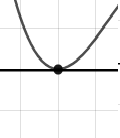
\includegraphics[width=0.3\textwidth]{../Figures/polyZeroBehaviorCC.png}
\end{center}\begin{enumerate}[label=\Alph*.]
\begin{multicols}{2}
\item 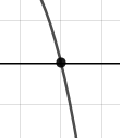
\includegraphics[width = 0.3\textwidth]{../Figures/polyZeroBehaviorAC.png}
\item 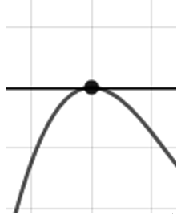
\includegraphics[width = 0.3\textwidth]{../Figures/polyZeroBehaviorBC.png}
\item 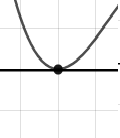
\includegraphics[width = 0.3\textwidth]{../Figures/polyZeroBehaviorCC.png}
\item 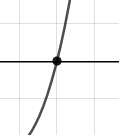
\includegraphics[width = 0.3\textwidth]{../Figures/polyZeroBehaviorDC.png}
\end{multicols}\item None of the above.\end{enumerate}
\textbf{General Comment:} You will need to sketch the entire graph, then zoom in on the zero the question asks about.
}
\litem{
Describe the zero behavior of the zero $x = -8$ of the polynomial below.
\[ f(x) = -8(x - 6)^{7}(x + 6)^{3}(x + 8)^{8}(x - 8)^{7} \]The solution is the graph below, which is option C.
\begin{center}
    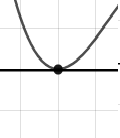
\includegraphics[width=0.3\textwidth]{../Figures/polyZeroBehaviorCopyCC.png}
\end{center}\begin{enumerate}[label=\Alph*.]
\begin{multicols}{2}
\item 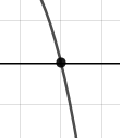
\includegraphics[width = 0.3\textwidth]{../Figures/polyZeroBehaviorCopyAC.png}
\item 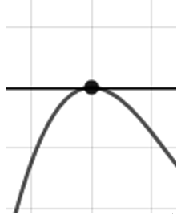
\includegraphics[width = 0.3\textwidth]{../Figures/polyZeroBehaviorCopyBC.png}
\item 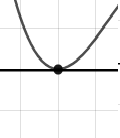
\includegraphics[width = 0.3\textwidth]{../Figures/polyZeroBehaviorCopyCC.png}
\item 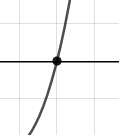
\includegraphics[width = 0.3\textwidth]{../Figures/polyZeroBehaviorCopyDC.png}
\end{multicols}\item None of the above.\end{enumerate}
\textbf{General Comment:} You will need to sketch the entire graph, then zoom in on the zero the question asks about.
}
\litem{
Which of the following equations \textit{could} be of the graph presented below?

\begin{center}
    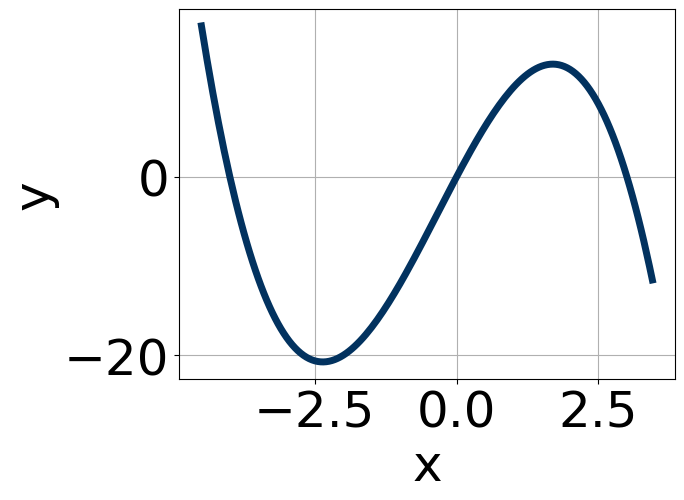
\includegraphics[width=0.5\textwidth]{../Figures/polyGraphToFunctionCopyC.png}
\end{center}


The solution is \( -8x^{9} (x + 4)^{9} (x - 3)^{7} \), which is option C.\begin{enumerate}[label=\Alph*.]
\item \( -17x^{9} (x + 4)^{6} (x - 3)^{11} \)

The factor $-4$ should have been an odd power.
\item \( -19x^{10} (x + 4)^{6} (x - 3)^{7} \)

The factors $-4$ and $0$ have have been odd power.
\item \( -8x^{9} (x + 4)^{9} (x - 3)^{7} \)

* This is the correct option.
\item \( 13x^{11} (x + 4)^{7} (x - 3)^{7} \)

This corresponds to the leading coefficient being the opposite value than it should be.
\item \( 16x^{7} (x + 4)^{10} (x - 3)^{9} \)

The factor $(x + 4)$ should have an odd power and the leading coefficient should be the opposite sign.
\end{enumerate}

\textbf{General Comment:} General Comments: Draw the x-axis to determine which zeros are touching (and so have even multiplicity) or cross (and have odd multiplicity).
}
\litem{
Describe the end behavior of the polynomial below.
\[ f(x) = -3(x + 5)^{5}(x - 5)^{8}(x + 9)^{2}(x - 9)^{3} \]The solution is the graph below, which is option B.
\begin{center}
    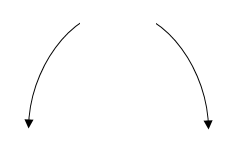
\includegraphics[width=0.3\textwidth]{../Figures/polyEndBehaviorBC.png}
\end{center}\begin{enumerate}[label=\Alph*.]
\begin{multicols}{2}
\item 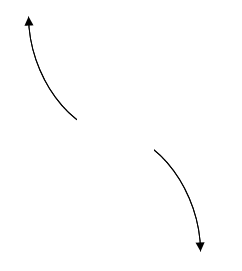
\includegraphics[width = 0.3\textwidth]{../Figures/polyEndBehaviorAC.png}
\item 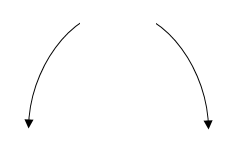
\includegraphics[width = 0.3\textwidth]{../Figures/polyEndBehaviorBC.png}
\item 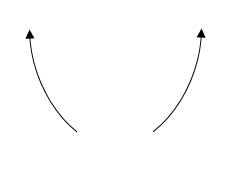
\includegraphics[width = 0.3\textwidth]{../Figures/polyEndBehaviorCC.png}
\item 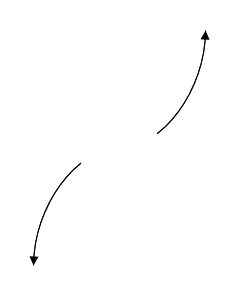
\includegraphics[width = 0.3\textwidth]{../Figures/polyEndBehaviorDC.png}
\end{multicols}\item None of the above.\end{enumerate}
\textbf{General Comment:} Remember that end behavior is determined by the leading coefficient AND whether the \textbf{sum} of the multiplicities is positive or negative.
}
\litem{
Construct the lowest-degree polynomial given the zeros below. Then, choose the intervals that contain the coefficients of the polynomial in the form $x^3+bx^2+cx+d$.
\[ 4 - 3 i \text{ and } -1 \]The solution is \( x^{3} -7 x^{2} +17 x + 25 \), which is option B.\begin{enumerate}[label=\Alph*.]
\item \( b \in [6, 11], c \in [16, 18], \text{ and } d \in [-26, -24] \)

$x^{3} +7 x^{2} +17 x -25$, which corresponds to multiplying out $(x-(4 - 3 i))(x-(4 + 3 i))(x -1)$.
\item \( b \in [-9, -4], c \in [16, 18], \text{ and } d \in [20, 28] \)

* $x^{3} -7 x^{2} +17 x + 25$, which is the correct option.
\item \( b \in [-2, 6], c \in [-4, -2], \text{ and } d \in [-4, -1] \)

$x^{3} + x^{2} -3 x -4$, which corresponds to multiplying out $(x -4)(x + 1)$.
\item \( b \in [-2, 6], c \in [3, 5], \text{ and } d \in [-1, 8] \)

$x^{3} + x^{2} +4 x + 3$, which corresponds to multiplying out $(x + 3)(x + 1)$.
\item \( \text{None of the above.} \)

This corresponds to making an unanticipated error or not understanding how to use nonreal complex numbers to create the lowest-degree polynomial. If you chose this and are not sure what you did wrong, please contact the coordinator for help.
\end{enumerate}

\textbf{General Comment:} Remember that the conjugate of $a+bi$ is $a-bi$. Since these zeros always come in pairs, we need to multiply out $(x-(4 - 3 i))(x-(4 + 3 i))(x-(-1))$.
}
\litem{
Construct the lowest-degree polynomial given the zeros below. Then, choose the intervals that contain the coefficients of the polynomial in the form $ax^3+bx^2+cx+d$.
\[ \frac{-2}{3}, \frac{-1}{4}, \text{ and } \frac{7}{4} \]The solution is \( 48x^{3} -40 x^{2} -69 x -14 \), which is option B.\begin{enumerate}[label=\Alph*.]
\item \( a \in [44, 54], b \in [-110, -98], c \in [21, 29], \text{ and } d \in [9, 22] \)

$48x^{3} -104 x^{2} +27 x + 14$, which corresponds to multiplying out $(3x -2)(4x + 1)(4x -7)$.
\item \( a \in [44, 54], b \in [-41, -35], c \in [-74, -64], \text{ and } d \in [-15, -11] \)

* $48x^{3} -40 x^{2} -69 x -14$, which is the correct option.
\item \( a \in [44, 54], b \in [-41, -35], c \in [-74, -64], \text{ and } d \in [9, 22] \)

$48x^{3} -40 x^{2} -69 x + 14$, which corresponds to multiplying everything correctly except the constant term.
\item \( a \in [44, 54], b \in [-134, -124], c \in [85, 86], \text{ and } d \in [-15, -11] \)

$48x^{3} -128 x^{2} +85 x -14$, which corresponds to multiplying out $(3x -2)(4x -1)(4x -7)$.
\item \( a \in [44, 54], b \in [40, 42], c \in [-74, -64], \text{ and } d \in [9, 22] \)

$48x^{3} +40 x^{2} -69 x + 14$, which corresponds to multiplying out $(3x -2)(4x -1)(4x + 7)$.
\end{enumerate}

\textbf{General Comment:} To construct the lowest-degree polynomial, you want to multiply out $(3x + 2)(4x + 1)(4x -7)$
}
\litem{
Describe the end behavior of the polynomial below.
\[ f(x) = 3(x - 3)^{2}(x + 3)^{7}(x + 9)^{5}(x - 9)^{7} \]The solution is the graph below, which is option D.
\begin{center}
    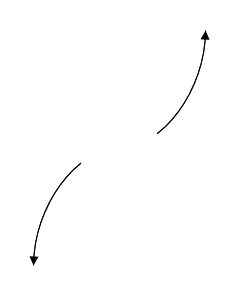
\includegraphics[width=0.3\textwidth]{../Figures/polyEndBehaviorCopyDC.png}
\end{center}\begin{enumerate}[label=\Alph*.]
\begin{multicols}{2}
\item 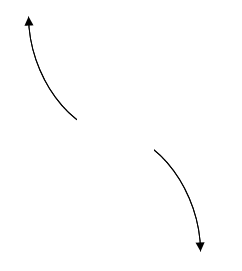
\includegraphics[width = 0.3\textwidth]{../Figures/polyEndBehaviorCopyAC.png}
\item 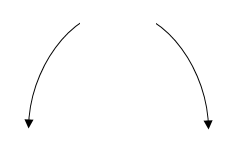
\includegraphics[width = 0.3\textwidth]{../Figures/polyEndBehaviorCopyBC.png}
\item 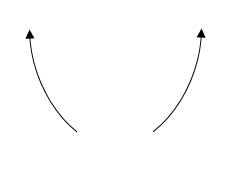
\includegraphics[width = 0.3\textwidth]{../Figures/polyEndBehaviorCopyCC.png}
\item 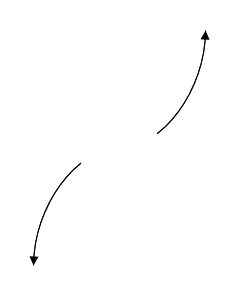
\includegraphics[width = 0.3\textwidth]{../Figures/polyEndBehaviorCopyDC.png}
\end{multicols}\item None of the above.\end{enumerate}
\textbf{General Comment:} Remember that end behavior is determined by the leading coefficient AND whether the \textbf{sum} of the multiplicities is positive or negative.
}
\litem{
Which of the following equations \textit{could} be of the graph presented below?

\begin{center}
    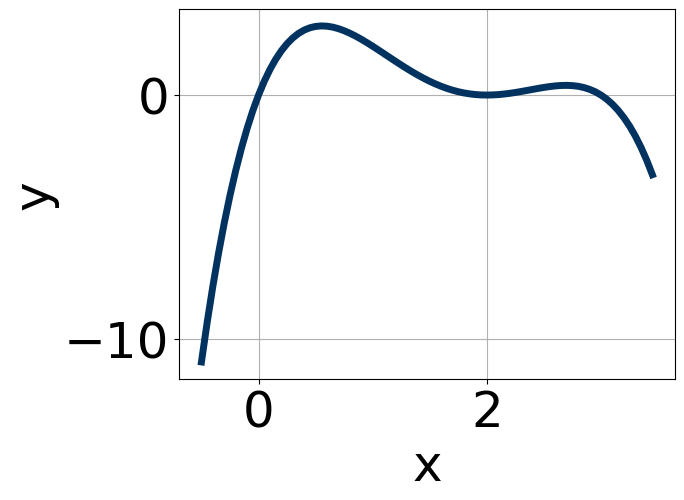
\includegraphics[width=0.5\textwidth]{../Figures/polyGraphToFunctionC.png}
\end{center}


The solution is \( 4(x - 1)^{11} (x - 3)^{11} (x + 4)^{9} \), which is option E.\begin{enumerate}[label=\Alph*.]
\item \( 17(x - 1)^{10} (x - 3)^{6} (x + 4)^{11} \)

The factors $1$ and $3$ have have been odd power.
\item \( -20(x - 1)^{10} (x - 3)^{11} (x + 4)^{11} \)

The factor $(x - 1)$ should have an odd power and the leading coefficient should be the opposite sign.
\item \( 4(x - 1)^{8} (x - 3)^{11} (x + 4)^{5} \)

The factor $1$ should have been an odd power.
\item \( -20(x - 1)^{11} (x - 3)^{5} (x + 4)^{5} \)

This corresponds to the leading coefficient being the opposite value than it should be.
\item \( 4(x - 1)^{11} (x - 3)^{11} (x + 4)^{9} \)

* This is the correct option.
\end{enumerate}

\textbf{General Comment:} General Comments: Draw the x-axis to determine which zeros are touching (and so have even multiplicity) or cross (and have odd multiplicity).
}
\end{enumerate}

\end{document}